\documentclass{standalone}
\usepackage{tikz}
\usetikzlibrary{patterns, positioning}


\begin{document}
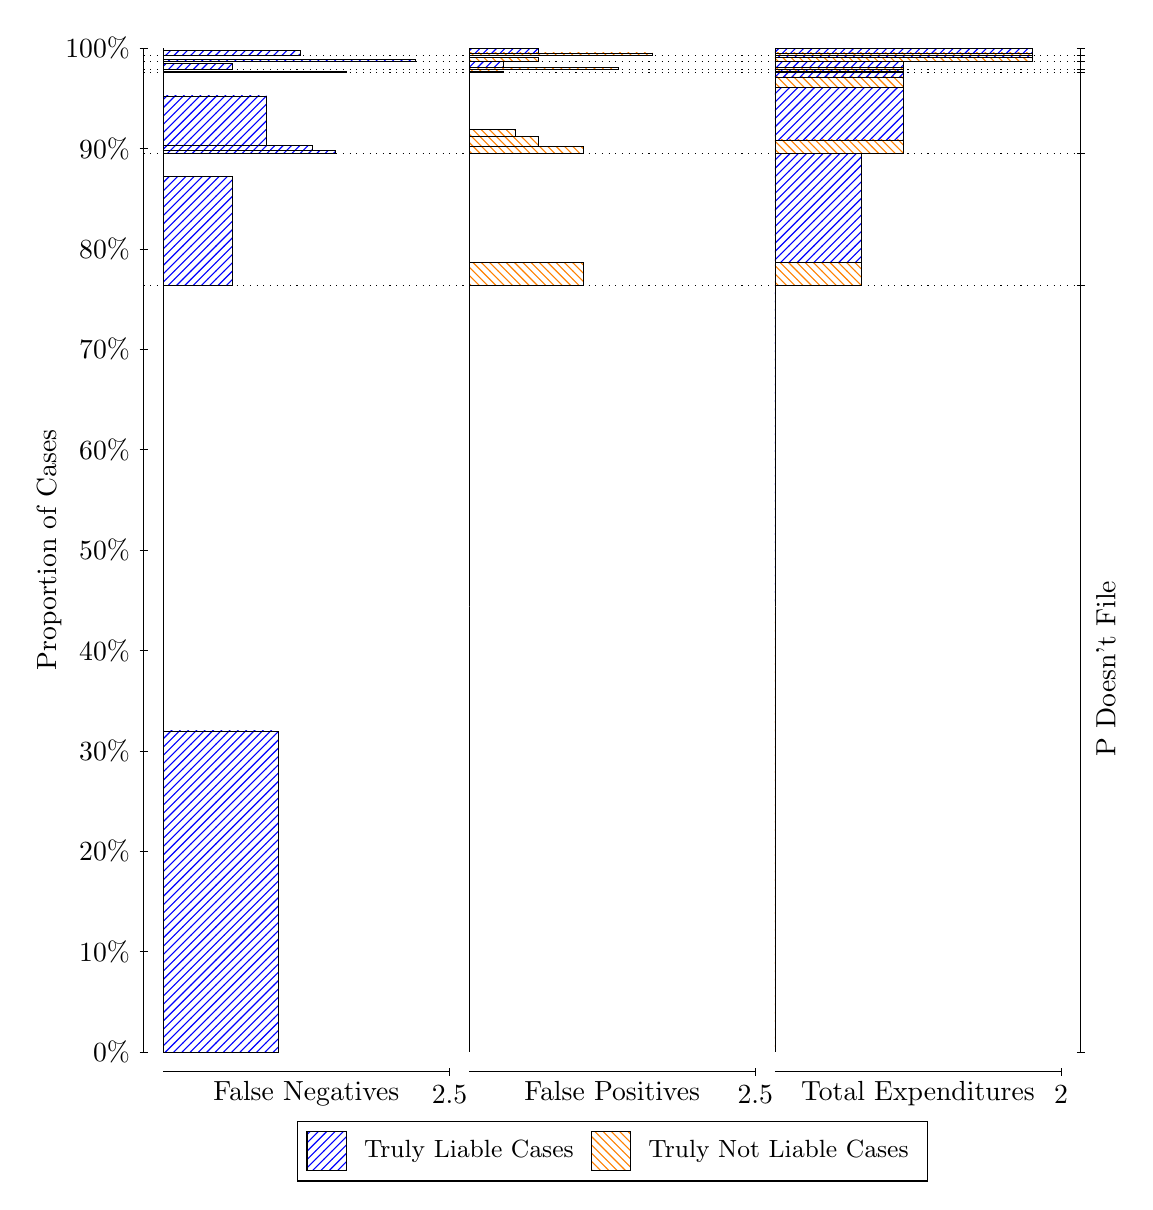
\begin{tikzpicture}
\draw[black, very thin] (1.5,1.75) -- (1.5,14.5);
\node[rotate=90, text=black, anchor=center] at (0.3, 8.125) {Proportion of Cases};
\draw[black, very thin] (1.45,1.75) -- (1.55,1.75);
\node[text=black, anchor=east] at (1.45, 1.75) {0\%};
\draw[black, very thin] (1.45,3.025) -- (1.55,3.025);
\node[text=black, anchor=east] at (1.45, 3.025) {10\%};
\draw[black, very thin] (1.45,4.3) -- (1.55,4.3);
\node[text=black, anchor=east] at (1.45, 4.3) {20\%};
\draw[black, very thin] (1.45,5.575) -- (1.55,5.575);
\node[text=black, anchor=east] at (1.45, 5.575) {30\%};
\draw[black, very thin] (1.45,6.85) -- (1.55,6.85);
\node[text=black, anchor=east] at (1.45, 6.85) {40\%};
\draw[black, very thin] (1.45,8.125) -- (1.55,8.125);
\node[text=black, anchor=east] at (1.45, 8.125) {50\%};
\draw[black, very thin] (1.45,9.4) -- (1.55,9.4);
\node[text=black, anchor=east] at (1.45, 9.4) {60\%};
\draw[black, very thin] (1.45,10.675) -- (1.55,10.675);
\node[text=black, anchor=east] at (1.45, 10.675) {70\%};
\draw[black, very thin] (1.45,11.95) -- (1.55,11.95);
\node[text=black, anchor=east] at (1.45, 11.95) {80\%};
\draw[black, very thin] (1.45,13.225) -- (1.55,13.225);
\node[text=black, anchor=east] at (1.45, 13.225) {90\%};
\draw[black, very thin] (1.45,14.5) -- (1.55,14.5);
\node[text=black, anchor=east] at (1.45, 14.5) {100\%};

\draw[black, very thin] (13.4,1.75) -- (13.4,14.5);
\draw[black, very thin] (13.35,1.75) -- (13.45,1.75);
\node[anchor=west] at (13.35, 1.75) {};
\draw[black, very thin] (13.35,11.486) -- (13.45,11.486);
\node[anchor=west] at (13.35, 11.486) {};
\draw[black, very thin] (13.35,13.163) -- (13.45,13.163);
\node[anchor=west] at (13.35, 13.163) {};
\draw[black, very thin] (13.35,14.193) -- (13.45,14.193);
\node[anchor=west] at (13.35, 14.193) {};
\draw[black, very thin] (13.35,14.226) -- (13.45,14.226);
\node[anchor=west] at (13.35, 14.226) {};
\draw[black, very thin] (13.35,14.326) -- (13.45,14.326);
\node[anchor=west] at (13.35, 14.326) {};
\draw[black, very thin] (13.35,14.408) -- (13.45,14.408);
\node[anchor=west] at (13.35, 14.408) {};
\draw[black, very thin] (13.35,14.5) -- (13.45,14.5);
\node[anchor=west] at (13.35, 14.5) {};

\draw[black, very thin, pattern color=blue, pattern=north east lines] (1.75,1.75) rectangle (3.2033,5.8268);
\draw[black, very thin, pattern color=orange, pattern=north west lines] (1.75,5.8268) rectangle (1.75,11.486);
\draw[black, very thin, pattern color=blue, pattern=north east lines] (1.75,11.486) rectangle (2.622,12.872);
\draw[black, very thin, pattern color=orange, pattern=north west lines] (1.75,12.872) rectangle (1.75,13.163);
\draw[black, very thin, pattern color=blue, pattern=north east lines] (1.75,13.163) rectangle (3.93,13.2);
\draw[black, very thin, pattern color=blue, pattern=north east lines] (1.75,13.2) rectangle (3.6393,13.26);
\draw[black, very thin, pattern color=blue, pattern=north east lines] (1.75,13.26) rectangle (3.058,13.893);
\draw[black, very thin, pattern color=orange, pattern=north west lines] (1.75,13.893) rectangle (1.75,14.193);
\draw[black, very thin, pattern color=blue, pattern=north east lines] (1.75,14.193) rectangle (4.0753,14.208);
\draw[black, very thin, pattern color=orange, pattern=north west lines] (1.75,14.208) rectangle (1.75,14.226);
\draw[black, very thin, pattern color=blue, pattern=north east lines] (1.75,14.226) rectangle (2.622,14.3);
\draw[black, very thin, pattern color=orange, pattern=north west lines] (1.75,14.3) rectangle (1.75,14.326);
\draw[black, very thin, pattern color=blue, pattern=north east lines] (1.75,14.326) rectangle (4.9473,14.356);
\draw[black, very thin, pattern color=orange, pattern=north west lines] (1.75,14.356) rectangle (1.75,14.408);
\draw[black, very thin, pattern color=blue, pattern=north east lines] (1.75,14.408) rectangle (3.494,14.47);
\draw[black, very thin, pattern color=orange, pattern=north west lines] (1.75,14.47) rectangle (1.75,14.5);
\draw[black, very thin, pattern color=orange, pattern=north west lines] (5.6333,1.75) rectangle (5.6333,7.4089);
\draw[black, very thin, pattern color=blue, pattern=north east lines] (5.6333,7.4089) rectangle (5.6333,11.486);
\draw[black, very thin, pattern color=orange, pattern=north west lines] (5.6333,11.486) rectangle (7.0867,11.777);
\draw[black, very thin, pattern color=blue, pattern=north east lines] (5.6333,11.777) rectangle (5.6333,13.163);
\draw[black, very thin, pattern color=orange, pattern=north west lines] (5.6333,13.163) rectangle (7.0867,13.247);
\draw[black, very thin, pattern color=orange, pattern=north west lines] (5.6333,13.247) rectangle (6.5053,13.377);
\draw[black, very thin, pattern color=orange, pattern=north west lines] (5.6333,13.377) rectangle (6.2147,13.462);
\draw[black, very thin, pattern color=blue, pattern=north east lines] (5.6333,13.462) rectangle (5.6333,14.193);
\draw[black, very thin, pattern color=orange, pattern=north west lines] (5.6333,14.193) rectangle (6.0693,14.21);
\draw[black, very thin, pattern color=blue, pattern=north east lines] (5.6333,14.21) rectangle (5.6333,14.226);
\draw[black, very thin, pattern color=orange, pattern=north west lines] (5.6333,14.226) rectangle (7.5227,14.252);
\draw[black, very thin, pattern color=blue, pattern=north east lines] (5.6333,14.252) rectangle (6.0693,14.326);
\draw[black, very thin, pattern color=orange, pattern=north west lines] (5.6333,14.326) rectangle (6.5053,14.378);
\draw[black, very thin, pattern color=blue, pattern=north east lines] (5.6333,14.378) rectangle (5.6333,14.408);
\draw[black, very thin, pattern color=orange, pattern=north west lines] (5.6333,14.408) rectangle (7.9587,14.438);
\draw[black, very thin, pattern color=blue, pattern=north east lines] (5.6333,14.438) rectangle (6.5053,14.5);
\draw[black, very thin, pattern color=orange, pattern=north west lines] (9.5167,1.75) rectangle (9.5167,7.4089);
\draw[black, very thin, pattern color=blue, pattern=north east lines] (9.5167,7.4089) rectangle (9.5167,11.486);
\draw[black, very thin, pattern color=orange, pattern=north west lines] (9.5167,11.486) rectangle (10.607,11.777);
\draw[black, very thin, pattern color=blue, pattern=north east lines] (9.5167,11.777) rectangle (10.607,13.163);
\draw[black, very thin, pattern color=orange, pattern=north west lines] (9.5167,13.163) rectangle (11.152,13.332);
\draw[black, very thin, pattern color=blue, pattern=north east lines] (9.5167,13.332) rectangle (11.152,14.002);
\draw[black, very thin, pattern color=orange, pattern=north west lines] (9.5167,14.002) rectangle (11.152,14.133);
\draw[black, very thin, pattern color=blue, pattern=north east lines] (9.5167,14.133) rectangle (11.152,14.193);
\draw[black, very thin, pattern color=orange, pattern=north west lines] (9.5167,14.193) rectangle (11.152,14.21);
\draw[black, very thin, pattern color=blue, pattern=north east lines] (9.5167,14.21) rectangle (11.152,14.226);
\draw[black, very thin, pattern color=orange, pattern=north west lines] (9.5167,14.226) rectangle (11.152,14.252);
\draw[black, very thin, pattern color=blue, pattern=north east lines] (9.5167,14.252) rectangle (11.152,14.326);
\draw[black, very thin, pattern color=orange, pattern=north west lines] (9.5167,14.326) rectangle (12.787,14.378);
\draw[black, very thin, pattern color=blue, pattern=north east lines] (9.5167,14.378) rectangle (12.787,14.408);
\draw[black, very thin, pattern color=orange, pattern=north west lines] (9.5167,14.408) rectangle (12.787,14.438);
\draw[black, very thin, pattern color=blue, pattern=north east lines] (9.5167,14.438) rectangle (12.787,14.5);
\draw[black, dotted] (1.5,11.486) -- (13.4,11.486);
\draw[black, dotted] (1.5,13.163) -- (13.4,13.163);
\draw[black, dotted] (1.5,14.193) -- (13.4,14.193);
\draw[black, dotted] (1.5,14.226) -- (13.4,14.226);
\draw[black, dotted] (1.5,14.326) -- (13.4,14.326);
\draw[black, dotted] (1.5,14.408) -- (13.4,14.408);
\draw[black, very thin] (1.75,1.5) -- (5.3833,1.5);
\node[text=black, anchor=north] at (3.5667, 1.5) {False Negatives};
\draw[black, very thin] (5.3833,1.45) -- (5.3833,1.55);
\node[text=black, anchor=north] at (5.3833, 1.45) {2.5};

\draw[black, very thin] (5.6333,1.5) -- (9.2667,1.5);
\node[text=black, anchor=north] at (7.45, 1.5) {False Positives};
\draw[black, very thin] (9.2667,1.45) -- (9.2667,1.55);
\node[text=black, anchor=north] at (9.2667, 1.45) {2.5};

\draw[black, very thin] (9.5167,1.5) -- (13.15,1.5);
\node[text=black, anchor=north] at (11.333, 1.5) {Total Expenditures};
\draw[black, very thin] (13.15,1.45) -- (13.15,1.55);
\node[text=black, anchor=north] at (13.15, 1.45) {2};

\node[text=black, centered, rotate=90] at (13.72, 6.6178) {P Doesn't File};







\draw (7.449999999999999,1.5) node[draw=none] (baseCoordinate) {};
\begin{scope}[align=center]
        \matrix[scale=0.5, draw=black, below=0.5cm of baseCoordinate, nodes={draw}, column sep=0.1cm]{
            \node[rectangle, draw, minimum width=0.5cm, minimum height=0.5cm, pattern color=blue, pattern=north east lines] {}; &
            \node[draw=none, font=\small, text=black] (B) {Truly Liable Cases}; &
            \node[rectangle, draw, minimum width=0.5cm, minimum height=0.5cm, pattern color=orange, pattern=north west lines] {}; &
            \node[draw=none, font=\small, text=black] (B) {Truly Not Liable Cases}; \\
            };
\end{scope}

\end{tikzpicture}
\end{document}